\documentclass[a4paper]{article}

\usepackage[a4paper, total={6in, 9.5in}]{geometry}
\usepackage[utf8]{inputenc}
\usepackage[T1]{fontenc}
\usepackage[british]{babel}
\usepackage{hyperref}
\usepackage[gen]{eurosym}
\usepackage{float}
\usepackage{mathtools}
\usepackage{amssymb}
\usepackage{enumitem}
\usepackage{lastpage}
\usepackage{multirow}
\usepackage{fancyhdr}
\usepackage{listings}

\usepackage{graphicx}
\graphicspath{{images/}}

\usepackage{xcolor}
\lstset{basicstyle=\ttfamily,
  showstringspaces=false,
  commentstyle=\color{red},
  keywordstyle=\color{blue}
}

\usepackage{titlesec}

\setcounter{secnumdepth}{4}

\titleformat{\paragraph}
{\normalfont\normalsize\bfseries}{\theparagraph}{1em}{}
\titlespacing*{\paragraph}
{0pt}{3.25ex plus 1ex minus .2ex}{1.5ex plus .2ex}


\usepackage{color}
\definecolor{gray97}{gray}{.97}
\definecolor{gray75}{gray}{.75}
\definecolor{gray45}{gray}{.45}
\definecolor{pblue}{rgb}{0.13,0.13,1}
\definecolor{pgreen}{rgb}{0,0.5,0}
\definecolor{pred}{rgb}{0.9,0,0}
\definecolor{pgrey}{rgb}{0.46,0.45,0.48}

\usepackage{listings}
\lstset{framerule=0pt,
	aboveskip=0.5cm,
	framextopmargin=3pt,
	framexbottommargin=3pt,
	framexleftmargin=0.4cm,
	framesep=0pt,
	rulesep=0.4pt,
	backgroundcolor=\color{gray97},
	rulesepcolor=\color{black},
	texcl=true,
	stringstyle=\ttfamily,
	%
	basicstyle=\ttfamily,
	keywordstyle=\color{blue}\ttfamily,
	stringstyle=\color{red}\ttfamily,
	commentstyle=\color{pgreen}\ttfamily,
	morecomment=[l][\color{magenta}]{\#}
	%
	numbers=left,
	numbersep=15pt,
	numberstyle=\scriptsize,
	numberfirstline=false,
	breaklines=true,
  	postbreak=\mbox{\textcolor{red}{$\hookrightarrow$}\space},
  	columns=fullflexible,
}

\lstnewenvironment{listing}[1][]
	{\lstset{#1}\pagebreak[0]}{\pagebreak[0]}
\lstdefinestyle{consola}
	{basicstyle=\scriptsize\bf\ttfamily,
		backgroundcolor=\color{gray75},
	}
\lstdefinestyle{C++}
	{language=C++,
	}


\pagestyle{fancy}

\lhead{Programación Declarativa}
\rhead{Página \thepage\ de \pageref{LastPage}}


\usepackage{parskip}
\begin{document}
\renewcommand{\contentsname}{Índice}

\begin{titlepage}
\begin{center}


\includegraphics[width=0.6\textwidth]{logoesi}\\[5cm]

% Title
\rule{\linewidth}{0.5mm} \\[0.4cm]
{ \huge \bfseries Programación Declarativa\\[0.4cm] }
\rule{\linewidth}{0.5mm} \\[1.5cm]
{\huge Interfaz \texttt{SWI-Prolog $\longleftrightarrow$ C/C++} (2017/2018)}\\[0.5cm]

% Authors
\large{Javier Córdoba Romero}\\
\large{Juan José Corroto Martín}\\

\end{center}
\end{titlepage}

\tableofcontents
\clearpage

\section{Introducción}

Este documento explica cómo utilizar las interfaces de SWI-Prolog con el lenguaje C[1] y con el lenguaje C++[2], para crear funciones en dichos lenguajes que puedan ser llamados desde un programa Prolog, del mismo modo que se llamaría a un predicado de Prolog y de forma transparente.

Estas funciones y predicados externos se realizan sobre la interfaz que SWI-Prolog nos proporciona, tanto en C como en C++, con una gran cantidad de tipos y funciones para manipular los tipos de Prolog, así como comunicarse con el núcleo de Prolog.

Este documento se centrará especialmente en la librería interfaz con el lenguaje C, y después se hará una comparación menos exhaustiva con la librería interfaz de C++, centrándonos especialmente en sus diferencias, ventajas y desventajas de cada una de ellas.
\subsection{Bibliotecas estáticas y dinámicas}

Los predicados externos que se quieran utilizar en Prolog deben agruparse en una librería externa. Estas librerías pueden ser:

\begin{itemize}
\item \textbf{Librería estática}. Las librerías estáticas se enlazan al fichero Prolog en tiempo de compilación, de manera que el archivo resultado de compilar los predicados externos consiste en un ejecutable que contiene tanto a dichos predicados como el núcleo de Prolog. De esta forma todos los predicados externos que hayamos definido en nuestro lenguaje de elección ya forman parte del entorno, y no es necesario cargarlos a posteriori.
\item \textbf{Librería dinámica}. Las librerías dinámicas se enlazan en tiempo de ejecución, y no de compilación. Esto quiere decir que el resultado de compilar nuestros predicados externos consistirá en un archivo con extensión de librería dinámica (En un Sistema Operativo Linux tendrán la extensión \textit{.so}, y en un Sistema Operativo tendrán extensión \textit{.dll}). Este fichero deberá cargarse desde un entorno de Prolog en funcionamiento con el predicado de SWI-Prolog   \textit{load\_foreign\_library/1}, cuyo argumento es el nombre de la librería.
\end{itemize}

Desde el punto de vista de la implementación de nuestros predicados externos, no influye la elección del tipo de librería que queramos desarrollar. El código fuente no cambiará.

En este documento se discutirán solo la creación de librerías dinámicas para SWI-Prolog.
\subsection{Predicados deterministas y no deterministas}

SWI-Prolog permite la implementación de predicados externos deterministas y no deterministas. Los predicados deterministas son aquellos que no permiten puntos de elección y sólo tienen éxito una vez, mientras que los no deterministas permiten varios puntos de elección, y pueden tener éxito al ser reevaluados en otro punto de elección. Sin embargo, nosotros sólo nos centraremos en la implementación de predicados deterministas, puesto que los predicados externos no deterministas son mucho más complejos, puesto que necesitan mantener información del contexto entre las diferentes llamadas al predicado externo para computar todas sus soluciones.


\section{Compilación, ejecución y depuración de bibliotecas dinámicas}

Antes de mostrar cómo se implementan predicados externos en C y C++, vamos a ver primero el proceso de compilado y enlazado de las librerías generadas.
\subsection{C}
\subsubsection{Compilación}
El proceso de compilar una librería dinámica para usarla en \texttt{SWI-Prolog} pasa por usar el comando \texttt{swipl-l} que por defecto es instalado junto a \texttt{SWI-Prolog} cuya función es compilar y enlazar el código que le proporcionemos.
Para compilar será necesario ejecutar el siguiente comando

\texttt{swipl-ld -Iinclude/ -c code.c -o out.o}

En esencia, este comando es una interfaz con \texttt{gcc} el cual ayuda a localizar e incluir los archivos de cabecera de \texttt{SWI-Prolog}.

Para enlazar los archivos obtenidos de la compilación se usará el siguiente comando

\texttt{swipl-ld -shared -o library.so code1.o code2.o}

Donde \texttt{codeX.o} son todos los archivos compilados usando el comando anterior.

El resultado de ejecutar este comando es un archivo \texttt{.so} que utilizaremos para cargar la librería dentro de la línea de comandos de \texttt{SWI-Prolog}.

\subsubsection{Ejecución}
Para ejecutar la librería compilada anteriormente es necesario ejecutar \texttt{SWI-Prolog} en el mismo directorio en el que se encuentra la librería y ejecutar el predicado \texttt{load\_foreign\_library(+library)} donde \texttt{library} es la ruta de la librería externa ya compilada.

Una vez ejecutado el predicado todos los predicados definidos dentro de la librería están disponibles dentro de \texttt{SWI-Prolog} como si de un predicado nativo se tratase.

El predicado \texttt{load\_foreign\_library} se puede incluir en una directiva dentro de un fichero de código \texttt{Prolog} para automatizar la carga de la librería.

\subsection{C++11}
\subsubsection{Compilación}
En el caso de C++, la compilación se realiza de forma similar. En este caso, es necesario usar el enlazador de SWI-Prolog a la vez del compilador de C++ para que la compilación se realice correctamente.

swipl-ld -shared -ld g++ -cc-options[" -std=c++11"

En este caso se usa la flag -cc-options del enlazador de SWI-Prolog para indicarlo al compilador de C++ que use el estándar C++11, para poder utilizar sus librerías y sus punteros inteligentes.
\subsubsection{Ejecución}
La ejecución usando la interfaz de C++ es similar a la de C, porque ésta interfaz está basada en la de C. Aunque, como luego veremos, la interfaz de C++ no tenga función de instalación, la macro que se va a usar para definir predicados externos, realiza procesos transparentes al programador que generan dicho función de instalación. Debido a esto, el flujo de ejecución es similar.

\subsection{Depuración}
Para poder depurar la librería externa se debería compilar el núcleo de \texttt{SWI-Prolog} con símbolos de depuración lo cual no es trivial y depende en gran medida del sistema operativo y plataforma usada.

La solución que se ha alcanzado es implementar una funcion de depuración a nivel de preprocesador, similar a la función \texttt{printf}.

Esta función imprime por la salida estándar de error el mensaje que le pasemos como argumentos e incluso valores en tiempo de compilación.

De esta manera podemos habilitar y deshabilitar todos los mensajes de depuración cambiando el comando de compilación. Definiendo una macro en tiempo de compilación.

El código que habilitaría/deshabilitaría los mensajes en tiempo de compilación sería el siguiente:

\begin{lstlisting}[style=C++]
#ifdef DEBUG
	#define DEBUG_PRINT(...) dbgprintf(__FILE__, __LINE__, __VA_ARGS__)
#else
	#define DEBUG_PRINT(...) do {} while(0)
#endif
\end{lstlisting}

La función \texttt{dbgprintf} está definida de la siguiente forma:

\begin{lstlisting}[style=C++]
void dbgprintf(const char* source_file, int source_line, const char* format_string, ...)
{
    va_list args;
    va_start(args, format_string);

    fprintf(stderr, "%s:%d: ", source_file, source_line);
    vfprintf(stderr, format_string, args);

    va_end(args);

}
\end{lstlisting}

De esta forma, para habilitar los mensajes de depuración solo tendríamos que añadir al comando de compilación la opción \texttt{-DDEBUG}

La forma de imprimir un mensaje sería llamar a la función \texttt{DEBUG\_PRINT} como si de otra función de C se tratase.


\section{Implementación de predicados externos}

En esta sección se presentan las características que deben tener nuestras funciones para ser consideradas predicados externos, además de algunas de las funciones C más importantes de C y C++ para comunicarse con Prolog y manejar sus términos. Más información en los manuales de referencia [1][2].

Aunque no se discutirán todas las operaciones implementadas, el listado completo de todas las operaciones que la librería contiene, tanto en C como en C++, es el siguiente:

\begin{itemize}
\item \textbf{is\_squared(+Matriz)}. Devuelve verdadero si la matriz es cuadrada, y falso en caso contrario.
\item \textbf{same\_dimensions(+Matriz1, +Matriz2)}. Devuelve verdadero si matriz1 y matriz2 tienen el mismo número de filas y columnas, y falso en caso contrario.
\item \textbf{mat\_sum(+Matriz, -sum)}. Devuelve la suma de todos los elementos de la matriz.
\item \textbf{sum\_mat(+Matriz1, +Matriz2, -MatrizResultado)}. Devuelve la matriz resultado de sumar matriz1 con matriz2.
\item \textbf{res\_mat(+Matriz1, +Matriz2, -MatrizResultado)}. Devuelve la matriz resultado de restar matriz1 con matriz2.
\item \textbf{mult\_mat\_factor(+Matriz, +factor, -MatrizResultado)}. Devuelve la matriz resultado de multiplicar matriz1 por un número.
\item \textbf{mult\_mat(+Matriz1, +Matriz2, -MatrizResultado)}. Devuelve la matriz resultado de multiplicar matriz1 con matriz2.
\item \textbf{transpose\_mat(+Matriz, -MatrizResultado)}. Devuelve la matriz resultado de transponer la matriz de entrada.
\item \textbf{determinant\_mat(+Matriz, -Determinante)}. Devuelve el determinante de la matriz de entrada, si lo tiene.
\item \textbf{inv\_mat(+Matriz, -MatrizInversa)}. Devuelve la matriz inversa de la matriz de entrada, si la tiene.
\end{itemize}
\subsection{C}
\subsubsection{Definición de predicados externos}
Para definir un predicado externo es necesario definir una función que devuelva un valor del tipo \texttt{foreign\_t} y acepte valores del tipo \texttt{term\_t} los cuales son los argumentos del predicado que serán proporcionados dentro del entorno de \texttt{SWI-Prolog}. 

Cada función que definamos se corresponderá con un predicado externo en \texttt{SWI-Prolog}.

La forma de devolver el control a \texttt{SWI-Prolog} es usar las macros \texttt{PL\_succeed} y \texttt{PL\_fail} que a su vez devuelven las macros \texttt{TRUE} y \texttt{FALSE}, cuyos valores son $1$ y $0$.

\subsubsection{Función de instalación}
Para que los predicados definidos en la librería externa estén disponible en \texttt{SWI-Prolog} es necesario definir una función de instalación que registre todos los predicados definidos en el núcleo de \texttt{SWI-Prolog}.

Esta función :
\begin{itemize}
	\item Tiene un tipo de retorno \texttt{install\_t}.
	\item No tiene parámetros de entrada.
	\item El nombre de la función es \texttt{install} o \texttt{install\_} seguido por el nombre de la biblioteca.
\end{itemize}

La función para registrar los predicados externos es

\texttt{PL\_register\_foreign(+name, +arity, +function, 0)}

El significado de estos argumentos son:
Esta función :
\begin{itemize}
	\item \textbf{+name} El nombre del predicado con el cual será llamado dentro de \texttt{SWI-Prolog}
	\item \textbf{+arity} El número de argumentos del predicado externo, que debe coincidir con el número de argumentos de la función definida en C
	\item \textbf{+function} El nombre de la función en código C, que no tiene por qué coincidir con el nombre del predicado que se usará en \texttt{SWI-Prolog}
\end{itemize}

Un ejemplo de definición de predicados y de función de instalación podría ser la implementación de un predicado que sumase dos números enteros:

\begin{lstlisting}[style=C++]
foreign_t
pl_sum_num(term_t n1, term_t n2, term_t res)
{
	int num1, num2 = 0;
	
	if (!PL_get_integer(n1, &num1)
		PL_fail;
	if (!PL_get_integer(n2, &num2)
		PL_fail;
	
	term_t r = PL_new_term_ref();
	
	return PL_put_integer(res, num1 + num2);
}

install_t
install()
{
	PL_register_foreign("sum_num", 2, pl_sum_num, 0);
}
\end{lstlisting}

\subsubsection{El tipo \texttt{term\_t}}
El tipo de datos \texttt{term\_t} es el principal tipo de datos en la librería externa de \texttt{SWI-Prolog}.

Este tipo de datos representa un puntero a un término de \texttt{SWI-Prolog} aunque este puntero no se puede manipular con los operadores habituales de C.

Los valores posibles de \texttt{term\_t} son:
\begin{itemize}
	\item Una variable.
	\item Un átomo.
	\item La constante \texttt{[]}, que representa el final de una lista.
	\item Datos binarios.
	\item Una cadena de texto.
	\item Un valor numérico.
	\item Un término compuesto
	\item Una lista.
	\item Un diccionario.
\end{itemize}

Las funciones más usadas para manejar términos son:
\begin{itemize}
	\item \textbf{PL\_new\_term\_ref()} Crea una referencia a un nuevo término.
	\item \textbf{PL\_new\_term\_refs(+count)} Crea \texttt{count} referencias a un nuevo término, estas referencias se pueden acceder sumando 1,2,3... al primer término.
	\item \textbf{PL\_copy\_term\_ref(+term)} Crea una referencia a un nuevo término el cual apunta inicialmente a \texttt{term}.
\end{itemize}

Una función muy interesante es \texttt{PL\_copy\_term\_ref} ya que permite recorrer una lista al estilo de \texttt{SWI-Prolog} un ejemplo es:

\begin{lstlisting}[style=C++]
foreign_t
pl_print_list(term_t list)
{
	if (!PL_is_list(list))
		PL_fail;
	
    term_t head = PL_new_term_ref();
    term_t tail = PL_copy_term_ref(list);
	
	while(PL_get_list(tail, head, tail))
	{
		char* str;
		PL_get_atom_chars(head, &str);
		
		printf("%s, ", str);
	}
	
	PL_succeed;
}
\end{lstlisting}

\subsubsection{Análisis y construcción de términos}
En la librería externa de \texttt{SWI-Prolog} existen diversas funciones que, permiten conocer qué tipo de variable está almacenado en una variable \texttt{term\_t} y que permiten relacionar esas variables con los tipos de C.
\paragraph{Comprobación de tipos}
La librería cuenta con una serie de funciones que permiten conocer el tipo de variable que contiene una variable \texttt{term\_t}.
Algunos de estos métodos son:
\begin{itemize}
	\item \texttt{PL\_is\_variable(+term)}
	\item \texttt{PL\_is\_atom(+term)}
	\item \texttt{PL\_is\_number(+term)}
	\item \texttt{PL\_is\_list(+term)}
	\item \texttt{PL\_is\_compound(+term)}
	\item \texttt{PL\_is\_string(+term)}
\end{itemize}

\paragraph{Términos simples}
La librería externa cuenta con funciones para obtener valores de los términos de \texttt{SWI-Prolog}, algunas de estas funciones son:
\begin{itemize}
	\item \texttt{PL\_get\_atom\_chars(+term, -char\_pointer)}
	\item \texttt{PL\_get\_integer(+term, -int\_pointer)}
	\item \texttt{PL\_get\_float(+term, -double\_pointer)}
\end{itemize}

También podemos usar funciones para guardar tipos de datos de C en un término de \texttt{SWI-Prolog}, algunas de estas funciones son:

\begin{itemize}
	\item \textbf{PL\_put\_variable(-term):} Que guarda una variable no inicializada en el término.
	\item \textbf{PL\_put\_atom\_chars(-term, +char\_pointer):} Que guarda una cadena de caracteres en el término.
	\item \textbf{PL\_put\_float(-term, +double):} Que guarda un número de punto flotante en el término.
\end{itemize}

Un ejemplo de operaciones con estas funciones sería la de sumar todos los elementos numéricos de una lista

\begin{lstlisting}[style=C++]
foreign_t
pl_sum_list(term_t list, term_t result)
{
	if (!PL_is_list(list))
		PL_fail;
	
	term_t head = PL_new_term_ref();
	term_t tail = PL_copy_term_ref(list);
	
	double sum = 0;
	
	while(PL_get_list(tail, head, tail))
	{
		double d = 0;
		int i = 0;
		if (!PL_is_number(head))
			continue;
		
		if (PL_is_integer(head))
		{
			PL_get_integer(head, &i);
			d = (double) i;
		}
		else
		{
			PL_get_float(head, &d);
		}
		
		sum += d;
	}
	
	term_t r = PL_new_term_ref();
	PL_put_float(result, sum);
}
\end{lstlisting}

\paragraph{Listas}
En la librería también existen funciones para crear, modificar y analizar listas de \texttt{SWI-Prolog}, algunas de estas funciones son:
\begin{itemize}
	\item \textbf{PL\_get\_list(+list, -head, -tail):} Que guarda en dos términos la cabeza y la cola de la lista correspondiente.
	\item \textbf{PL\_get\_nil(+list):} Comprueba si el término representa la constante de final de lista.
	\item \textbf{PL\_cons\_list(-list, +head, +tail):} Construye una lista nueva formada por la unión de la cabeza y la cola. La lista objetivo y la cola pueden ser el mismo término, lo que ayuda a construir listas en un bucle.
	\item \textbf{PL\_skip\_list(+list, -tail, -length):} Permite conocer la longitud de la lista y, a la vez, obtener un término que hace referencia al último elemento de la lista.
\end{itemize}

\subsubsection{Otras funciones}.
Otra función interesante dentro de la librería es la posibilidad de unificar dos términos de la misma forma que se produce la unificación en \texttt{SWI-Prolog}

Esta función es \texttt{PL\_unify(term1, term2)} que intenta unificar term2 con term1.

Para ejemplificar este apartado junto con el de listas se implementará un predicado externo que construya una lista de los que contenga todos los números naturales que hay entre los dos argumentos pasados al predicado, la lista resultante se unificará para que el predicado tenga también un propósito de comprobar si una lista genérica es la lista de elementos consecutivos entre dos números:

\begin{lstlisting}[style=C++]
foreign_t
pl_gen_list(term_t low, term_t high, term_t list)
{
	if (!PL_is_integer(low) || !PL_is_integer(high))
		PL_fail;
	
	int l, h;
	
	PL_get_integer(low, &l); // Get the numeric values of the terms
	PL_get_integer(high, &h);
	
	if (l > h || l < 0) // Check if the range is valid
		PL_fail;
	
	term_t res = PL_new_term_ref();
	PL_put_nil(res); // Put the empty list constant in the new term
	
	term_t num = PL_new_term_ref();
	
	for (int i = l; i <= h; i++)
	{
		PL_put_integer(num, i); // Put the numeric value on the term
		PL_cons_list(list, num, list); // Build the list tail-to-head
	}
	
	return PL_unify(list, res); // Unify with the list
}
\end{lstlisting}

\subsection{C++11}
\subsubsection{Definición de predicados externos}
Al igual que en C, una biblioteca externa puede tener tantos predicados externos como se desee. Cada uno de ellos estará asociado a un bloque de código. Ésta es la primera diferencia que tenemos con respecto a la interfaz con C, nuestros predicados no serán funciones C++, si no bloques de código. Sin embargo, el flujo de ejecución es el mismo que en la interfaz de C: después de cargar la librería dinámica mediante el predicado \textit{load\_foreign\_library/1}, e invocar uno de los predicados externos, se cede el control al bloque de código C++, que al finalizar, devuelve el control a Prolog.

Los bloques de código de C++ asociados a un predicado externo estarán marcados mediante la macro PREDICATE(name, arity). En esta macro se establece:

\begin{itemize}
\item El nombre del predicado que se invocará en Prolog.
\item La aridad, es decir, el número de argumentos que tomará el predicado.
\end{itemize}

Con esta macro ya hemos realizado toda la instalación del bloque de código, y ya puede ser llamado desde Prolog. En realidad, la macro lo que está haciendo por nosotros es envolver todo el boque de código designado mediante una función con tipo de retorno \textit{foreignt\_t}, con el número de argumentos que le hemos establecido de tipo PlTerm (más adelante aclararemos qué es este tipo), y también genera la función de instalación para este bloque. Esto quiere decir que no tenemos que preocuparnos por ninguno de estos temas cuando usemos dicha macro.

Estos bloque de código deberán retornar siempre TRUE, si el predicado ha tenido un resultado exitoso, o FALSE si ha fallado.

Además, podemos acceder a los argumentos de nuestro predicado mediante las macros $A_n$, siendo $n$ el número del argumento que accedemos. Por ejemplo, si queremos acceder al primer argumento, podemos acceder a él mediante $A_1$, variable de tipo PlTerm.

Ejemplo de predicado externo en el que se devuelve FALSE si la matriz pasada como argumento no es cuadrada, y TRUE si sí lo es:

\begin{lstlisting}[style=C++]
PREDICATE(is_squared, 1)
{
	std::unique_ptr<Matrix> m1(list_to_Matrix(A1));
	
	if (m1.get() == nullptr || !m1->isSquared())
	{
		return FALSE;
	}
	
	return TRUE;
}
\end{lstlisting}

Algunas de las funciones que aparecen en el ejemplo serán discutidas más adelante (como por ejemplo \textit{list\_to\_Matrix}).

\subsubsection{El tipo \texttt{PlTerm}}

En la interfaz de C++, que recordamos es totalmente compatible con la interfaz de C, tenemos a nuestra disposición un tipo más abstracto de datos que nos permite manipular términos de Prolog. Éste es el tipo $PlTerm$, una clase definida en la interfaz de C++. Las macros de nuestros argumentos $A_n$ son de este tipo.

Los tipos $PlTerm$ contienen una referencia a un término de prólog, al igual que el tipo \textit{term\_t}, pero nos da un nivel mayor de abstracción que más tarde discutiremos. 

En caso de que queramos construir un nuevo término de Prolog, podemos hacerlo mediante múltiple constructores a nuestra disposición, entre los que se incluyen:
\begin{itemize}
\item PlTerm::PlTerm(). Crea una nueva referencia a un término de Prolog sin inicializar.
\item PlTerm::PlTerm(\textit{term\_t}. Con el que podemos convertir un tipo de término de la interfaz de C a un tipo de la interfaz C++.
\item PlTErm::PlTerm(double d). Con el que podemos crear una referencia a un término de prolog que contiene el número en punto flotante d.
\end{itemize}

Además también tenemos el tipo $PlTermv$, que consiste en un vector de $PlTerm$. Este tipo tiene sobrecargado el operador ( ) para poder acceder a cualquier de los términos que contiene, empezando en 0. Sin embargo, este tipo es principalmente usado para pasar argumentos en llamadas desde C++ a Prolog. Esto será discutido más adelante.

Una de las cosas más importante que ofrece la clase $PlTerm$ es la sobrecarga del operador $=$. En el caso de que usemos el operador $=$ con un $PlTerm$, no estaremos asignando, sino unificando un valor con dicho término. Por lo tanto la operación $=$ devuelve un valor booleano verdadero si la unificación fue un éxito, o uno falso si la unificación falló. Esto es importante porque, al igual que en Prolog, una vez unificado un término dentro de nuestro predicado, no se puede volver a unificar con algo distinto. En este caso devolvería un valor falso y el bloque de código continuaría.

A continuación un ejemplo de creación de términos, así como uno de unificación.

\begin{lstlisting}[style=C++]
PlTerm term1(); //Crea una referencia vacía a un término

PlTerm term2(2.0); //Crea una referencia al término 2.0
\end{lstlisting}

\begin{lstlisting}[style=C++]
PREDICATE(mat_sum, 2)
{
    std::unique_ptr<Matrix> m1(list_to_Matrix(A1));
	
	if (m1.get() == nullptr)
	{
		return FALSE;
	}
	
	return A2 = m1->sum(); //Devolveremos verdadero si el término A2 se puede unificar con la suma de la matriz m1
}
\end{lstlisting}

\subsubsection{Casteo de tipos y excepciones}

Una de las cosas más potentes que nos ofrece la interfaz de C++ con respecto a la de C es el casteo de tipos. Esto consiste en convertir uno de nuestros términos $PlTerm$ en una valor de C++, como por ejemplo un valor en punto flotante. En el siguiente ejemplo se puede ver una instrucción perfectamente válida.

\begin{lstlisting}[style=C++]
PREDICATE(sum, 2)
{
	
	double value = (double) A1 + 2.0;
	
	PlTerm ret_term(value);
	
	return A2 = ret_term;
}
\end{lstlisting}

Sin embargo, los términos no tienen por qué ser un valor en punto flotante, por lo que el casteo fallaría. En este caso, las excepciones entran en juego.
En el caso anterior, si llamaramos al predicado sum/2 , siendo el primer argumento $a$, la instrucción $(double) A1$ lanzaría una excepción de tipo $PlTypeError$, excepción que se lanza cuando cualquier casteo falla. La interfaz además implementa más tipos de excepciones:

\begin{itemize}
\item PlTypeError: excepción lanzada cuando un termino no satisface el tipo esperado por Prolog. Como se ha definido antes, es el tipo que se lanza en el casteo fallido, pero también en otras llamadas a la interfaz que veremos más adelante.
\item PlDomainError: excepción lanzada cuando un termino satisface el tipo esperado de Prolog, pero no es aceptable para el dominio esperado por una operación. Por ejemplo, la llamada al predicado de Prolog open/3 espera un \textit{io\_mode}(leer, escribir, etc). Si se pasa como argumento un entero, es un error de tipo y se lanzaría la excepción PlTypeError. Sin embargo, si se pasa un átomo distinto a los \textit{io\_mode}, se lanza una PlDomainError.
\item PlException: Esta subclase de PlTerm actúa como clase padre de las demás excepciones, y nos permite definir nuestras propias excepciones. También la podemos usar como excepción general para capturar las excepciones lanzadas por Prolog en un bloque try-catch.
\end{itemize}

Es importante conocer que todas estas excepciones son lanzadas desde C++, y por tanto pueden ser controladas desde el mismo bloque de instrucciones que forma el predicado externo.

Ahora procedemos a realizar el mismo ejemplo que antes, pero esta vez cerciorándonos que controlamos todas los posibles escenarios.

\begin{lstlisting}[style=C++]
PREDICATE(sum, 2)
{
	try{
		double value = (double) A1 + 2.0;
	}
	catch (PlException &ex)
	{
		std::cout << "El primer termino debe ser un numero" << std::endl;
		return FALSE;
	}
	PlTerm ret_term(value);
	
	return A2 = ret_term;
}
\end{lstlisting}

En este nuevo predicado, si el usuario introduce como primer argumento un término que no sea un número, el casteo lanzará una excepción que capturaremos. Le comunicamos al usuario el error y devolvemos false, en lugar de dejar que Prolog cese su ejecución.

\subsubsection{El tipo \texttt{PlTail}}

La clase que la interfaz nos ofrece para manipular listas de prolog es $PlTail$. Este clase nos permite asignar una referencia una lista e iterar sobre ella. Algo importante a tener en cuenta es que el constructor:

\begin{lstlisting}[style=C++]
PlTail list(term);
\end{lstlisting}

Admite como parámetro un término del tipo PlTerm, pero este término debe ser ya una lista. Esto quiere decir que la interfaz no nos permite construir nuevas listas.

La clase PlTail contiene las siguientes operaciones:

\begin{itemize}
\item PlTail::append(PlTerm \&term). Añade un término a la lista, poniéndose este nuevo término como nueva cabeza de la lista.
\item PlTail::close(). Ésta función intenta unificar la lista con la lista vacía, devolviendo verdadero si la unificación ha tenido éxito, y falso en caso contrario.
\item PlTail::next(PlTerm \&term). Éste método nos permitirá iterar sobra la lista, asignando al término que pasamos como argumento una referencia a la cabeza de la lista, y haciendo que $PlTail$ apunte al siguiente elemento. Esto quiere decir que cuando iteramos sobre la lista, estamos consumiendo los elementos, por lo que al final la variable PlTail quedará apuntando a una lista vacía.
\end{itemize}

A continuación se presenta un ejemplo característico del uso del tipo PlTail.

\begin{lstlisting}[style=C++]
PlTail list(term);


PlTerm e1;

while (list.next(e1)) {
	content.push_back((double) e1);
}
\end{lstlisting}

En el ejemplo anterior, se puede ver como se construye una lista a partir de un término, y después se itera sobre la lista, asignando la referencia de la cabeza de la lista en cada iteración a un término sin inicializar. Después casteamos dicho término a un número en punto flotante y lo agregamos a un vector. 

Es importante tener en cuenta que si, en el ejemplo anterior, el término $term$ no fuese una lista, el constructor lanzaría una PlTypeError (excepción de tipo).
\subsubsection{Llamadas a predicados Prolog}

La interfaz de C++ también nos permite hacer llamadas a predicados de Prolog desde C++, pudiéndose así establecer una conversación entre sendos lenguajes.

Para esto, la interfaz nos da la clase $PlQuery$, que nos permite definir una consulta a un predicado Prolog, así como obtener sus soluciones.

los distintos constructores para la clase son los siguientes:
\begin{itemize}
\item PlQuery::PlQuery(const char* name, PlTermv \&av). Crea una consulta al predicado de nombre $name$, y le pasa como argumentos aquellos del vector $av$. La aridad del predicado que llamamos es deducida del vector de términos $av$, por lo que no tenemos que decírsela.
\item PlQuery::PlQuery(const char* module, const char* name, PlTermv \&av). Realiza la misma construcción que el anterior, pero esta vez podemos indicarle el nombre del módulo en el que el predicado se encuentra.
\end{itemize}

La función que utilizaremos para obtener soluciones es $PlQuery::next\_solution()$, que llama al predicado y obtiene en el vector de argumentos la siguiente solución, si la hay.

A continuación se presenta un ejemplo típico de uso:

\begin{lstlisting}[style=C++]
PREDICATE(average, 3)
{ long sum = 0;
  long n = 0;

  PlQuery q("call", PlTermv(A2));
  while( q.next_solution() )
  { sum += (long)A1;
    n++;
  }
  return A3 = (double)sum/(double)n;
}
\end{lstlisting}

En este ejemplo utilizamos el predicado de orden superior call/1, de tal modo que podemos calcular la media de las soluciones que el segundo argumento, un predicado, nos de.

\subsubsection{Construcción de una lista}

Aunque se ha discutido anteriormente, es importante resaltar que la interfaz de C++ no nos ofrece la posibilidad de construir nuevas listas. Esto es debido a que la clase de la que disponemos para manipular listas, $PlTail$, admite en su constructor un término que ya sea una lista. Para solventarlo, hemos aprovechado la compatibilidad tanto de los lenguajes C y C++ como de las interfaces de dichos lenguajes, y hemos invocado a la interfaz de C. De este modo, conseguimos un término \textit{term\_t} que contiene la lista, y éste es el que usamos para construir nuestro PlTerm que vamos a unificar con la solución. 

Las funciones utilizadas para la creación de esta lista ya han sido discutidas en la parte de C de este documento.

\section{Ejemplos}

En esta sección se va a presentar un ejemplo concreto y concreto de la biblioteca dinámica que hemos desarrollado. El ejemplo constará de los siguientes predicados externos:

\begin{itemize}
\item \textbf{sum\_mat(+Matriz1, +Matriz2, -MatrixResultado)}. Suma cada uno de los componentes de ambas matrices, y nos devuelve el resultado en una nueva matriz. Ejemplo:

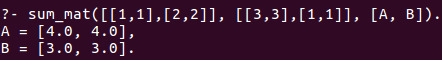
\includegraphics[scale=0.6]{EjemploSuma.jpeg}
\item \textbf{mult\_mat(+Matriz1, +Matriz2, -MatrixResultado)}. Realiza la multiplicación de matriz1 y matriz2 y nos devuelve el resultado en una nueva matriz. Ejemplo:

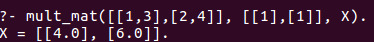
\includegraphics[scale=0.6]{EjemploMult.jpeg}
\end{itemize}

Además de estas operaciones, se han implementado multitud más de operaciones con matrices que se pueden encontrar en el código fuente adjunto, tanto en C como en C++.

El mayor esfuerzo ha sido situado en la comprobación de tipos, de tal modo que los predicados sean capaces de admitir cualquier tipo de término de Prolog y lograr una respuesta, aunque se evalúe el predicado a falso, en vez de cortar la ejecución de Prolog.

\subsection{C}
Debido a la naturaleza de bajo nivel de C la lógica de la librería dinámica está mezclada con las comprobaciones de errores y el tratamiento de memoria dinámica, aun así se podrían distinguir 4 partes bien diferencias en un predicado externo:
\begin{itemize}
	\item \textbf{Comprobación-Conversión:} De los tipos de \texttt{SWI-Prolog} a tipos y estructuras de C.
	\item \textbf{Obtención de memoria dinámica:} Donde se guardará la matriz resultado.
	\item \textbf{Obtención:} Del resultado del predicado mediante operaciones definidas previamente
	\item \textbf{Conversión:} De tipos de datos C a valores de \texttt{SWI-Prolog}.
	\item \textbf{Liberación de memoria dinámica:} Para prevenir las fugas de memoria.
\end{itemize}
\subsubsection{sum\_mat}
El código que realiza la suma de matrices es:
\begin{lstlisting}[style=C++]
int add_matrices(const struct Matrix_t* m1, const struct Matrix_t* m2, struct Matrix_t* result)
{
    if (!m1)
        return 0;
    if (!m1->size)
        return 0;
    if (!m1->rows)
        return 0;

    if (!m2)
        return 0;
    if (!m2->size)
        return 0;
    if (!m2->rows)
        return 0;

    if (!result)
        return 0;
    if (!result->size)
        return 0;
    if (!result->rows)
        return 0;


    int same_dims = 0;
    if (!is_same_dimensions(m1, m2, &same_dims))
        return 0;

    if (!same_dims)
    	return 0;

    for (int i = 0; i < result->size[0]; i++)
    {
        for (int j = 0; j < result->size[1]; j++)
        {
            result->rows[i][j] = m1->rows[i][j] + m2->rows[i][j];
        }
    }

    return 1;
}
\end{lstlisting}

El código que realiza la traducción \texttt{SWI-Prolog $\longleftrightarrow$ C}:
\begin{lstlisting}[style=C++]
foreign_t
pl_add_matrices(term_t m1, term_t m2, term_t result)
{
	struct Matrix_t* matrix1;
	struct Matrix_t* matrix2;
	struct Matrix_t* mresult = NULL;

	matrix1 = list_to_matrix(m1);
	if (!matrix1)
		PL_fail;

	matrix2 = list_to_matrix(m2);
	if (!matrix2)
	{
		free_matrix(matrix1);
		PL_fail;
	}


	mresult = alloc_matrix(matrix1->size);
    if (!mresult)
    {
		free_matrix(matrix1); free_matrix(matrix2);
        PL_fail;
    }
	
	if (!add_matrices(matrix1, matrix2, mresult))
	{
		free_matrix(matrix1); free_matrix(matrix2); free_matrix(mresult);
        PL_fail;
	}

	term_t mlist = PL_new_term_ref();
	if (!matrix_to_list(mresult, mlist))
	{
		free_matrix(matrix1); free_matrix(matrix2); free_matrix(mresult);
        PL_fail;
	}
	
	if (!free_matrix(matrix1) | !free_matrix(matrix2) | !free_matrix(mresult))
		PL_fail;

	return PL_unify(result, mlist);
}
\end{lstlisting}

\subsubsection{mult\_mat}
El código que realiza la multiplicación de matrices es:
\begin{lstlisting}[style=C++]
int multiply_matrices(const struct Matrix_t* m1, const struct Matrix_t* m2, struct Matrix_t* result)
{
    if (!m1)
        return 0;
    if (!m1->size)
        return 0;
    if (!m1->rows)
        return 0;

    if (!m2)
        return 0;
    if (!m2->size)
        return 0;
    if (!m2->rows)
        return 0;

    if (!result)
        return 0;
    if (!result->size)
        return 0;
    if (!result->rows)
        return 0;


    if (m1->size[1] != m2->size[0])
    {
        return 0;
    }

    for (int i = 0; i < result->size[0]; i++)
    {
        for (int j = 0; j < result->size[1]; j++)
        {
            double res = 0;
            for (int k = 0; k < m1->size[1]; k++)
            {
                res += m1->rows[i][k] * m2->rows[k][j];
            }
            result->rows[i][j] = res;
        }
    }
    
    return 1;
}
\end{lstlisting}

El código que realiza la traducción \texttt{SWI-Prolog $\longleftrightarrow$ C}:
\begin{lstlisting}[style=C++]
foreign_t
pl_multiply_matrices(term_t m1, term_t m2, term_t result)
{
	struct Matrix_t* matrix1;
	struct Matrix_t* matrix2;
	struct Matrix_t* mresult = NULL;

	matrix1 = list_to_matrix(m1);
	if (!matrix1)
	{
		PL_fail;
	}

	matrix2 = list_to_matrix(m2);
	if (!matrix2)
	{
		free_matrix(matrix1);
		PL_fail;
	}

	size_t nsize[2] = {0};
	nsize[0] = matrix1->size[0];
	nsize[1] = matrix2->size[1];
	mresult = alloc_matrix(nsize);
    if (!mresult)
    {
		free_matrix(matrix1); free_matrix(matrix2);
        PL_fail;
    }
	
	if (!multiply_matrices(matrix1, matrix2, mresult))
	{
		DEBUG_PRINT("Cannot multiply matrices\n");
		free_matrix(matrix1); free_matrix(matrix2); free_matrix(mresult);
	}

	term_t mlist = PL_new_term_ref();
	if (!matrix_to_list(mresult, mlist))
	{
		free_matrix(matrix1); free_matrix(matrix2); free_matrix(mresult);
        PL_fail;
	}
	
	if (!free_matrix(matrix1) | !free_matrix(matrix2) | !free_matrix(mresult))
	{
		PL_fail;
	}

	return PL_unify(result, mlist);
}
\end{lstlisting}

\subsubsection{Matrix struct}
A continuación se detalla la la estructura que se usa para representar una matriz de \texttt{nxn} elementos:

\begin{lstlisting}[style=C++]
struct Matrix_t
{
    size_t size[2]; // Matrix dimensions

    double** rows; // Matrix rows
};
\end{lstlisting}


\subsubsection{Funciones auxiliares}
\subsubsection{\texttt{SWI-Prolog $\longrightarrow$ C}}
Para convertir una lista de \texttt{SWI-Prolog}, que representa una fila, en un array de C contamos con la siguiente funcion:
\begin{lstlisting}[style=C++]
int list_to_row(const term_t list, size_t length, double* row)
{
    if (!row)
        return 0;

    term_t head = PL_new_term_ref();
    term_t tail = PL_copy_term_ref(list);

    for (int i = 0; i < length; i++)
    {
        if (!PL_get_list(tail, head, tail))
            return 0;

        int ival;
        double dval;
        switch (PL_term_type(head))
        {
            case PL_INTEGER:
                if (!PL_get_integer(head, &ival))
                    return 0;

                *(row + i) = (double) ival;
                break;
            
            case PL_FLOAT:
                if (!PL_get_float(head, &dval))
                    return 0;

                *(row + i) = dval;
                break;

            default:
                return 0;
        }
    }
    
    return 1;
}
\end{lstlisting}

\subsubsection{\texttt{SWI-Prolog $\longleftarrow$ C}}
Para convertir un array de C, que representa una fila, en una lista de \texttt{SWI-Prolog} contamos con la siguiente funcion:
\begin{lstlisting}[style=C++]
int row_to_list(double* row, size_t length, term_t list)
{
    if (!row)
        return 0;

    PL_put_nil(list);

    term_t num = PL_new_term_ref();
    
    for (int i = length - 1; i >= 0; i--)
    {
        int res = PL_put_float(num, row[i]);
        if (res != TRUE)
            return 0;

        res = PL_cons_list(list, num, list);
        if (res != TRUE)
            return 0;
    }
    return 1;
}
\end{lstlisting}

También tenemos funciones que no convierten los tipos, si no que manejan la memoria que se asigna y se libera para mejorar la modularización y a prevenir errores relaciones con la gestión de la memoria:

la siguiente función reserva memoria para una matriz de tamaño \texttt{size}:
\begin{lstlisting}[style=C++]
struct Matrix_t* alloc_matrix(const size_t size[2])
{
    if (!size)
        return NULL;

    if (size[0] < 1 || size[1] < 1)
        return 0;

    struct Matrix_t* mat = calloc(1, sizeof(struct Matrix_t));
    if (!mat)
        return NULL;

    memcpy(mat->size, size, sizeof(size_t) * 2);


    int rows = size[0];
    int cols = size[1];

    double** rptr = (double**) calloc(rows, sizeof(double*));

    if (!rptr)
    {
        free(mat);
        mat = NULL;
        return NULL;
    }
    else
    {
        mat->rows = rptr;
    }

    for (int i = 0; i < rows; i++)
    {
        double* cptr = (double*) calloc(cols, sizeof(double));
        if (!cptr)
        {
            for (int j = 0; j < i; j++)
            {
                free(*(mat->rows + i));
                *(mat->rows + i) = NULL;
            }
            free(rptr);
            rptr = NULL;
            free(mat);
            mat = NULL;
            return NULL;
        }
        else
        {
            *(mat->rows + i) = cptr;
        }
    }

    return mat;
}
\end{lstlisting}

La siguiente función libera de la memoria un puntero a una estructura que almacena una matriz, es notable la comprobación para evitar liberar la misma dirección de memoria varias veces:
:
\begin{lstlisting}[style=C++]
int free_matrix(struct Matrix_t* matrix)
{
    if (!matrix)
        return 0;
    if (!matrix->size)
        return 0;

    for (int i = 0; i < matrix->size[0]; i++)
    {
        if (*(matrix->rows + i))
        {
            free(*(matrix->rows + i));
            *(matrix->rows + i) = NULL;
        }
    }

    free(matrix->rows);
    matrix->rows = NULL;
    
    free(matrix);
    matrix = NULL;
    
    return 1;
}
\end{lstlisting}

\subsection{C++}

En la librería dinámica de C++, se ha logrado una gran modularización de las responsabilidades, de tal manera que todos los predicados constan de tres partes bien diferenciadas:
\begin{itemize}
\item \textbf{Conversión} los tipos de Prolog en una clase definida en C++ de matrices.
\item \textbf{Obtención} de matriz resultado (u obtención de resultado en caso de que sea un predicado que devuelva un número), mediante operaciones propias de C++, utilizando la clase definida en C++.
\item \textbf{Contrucción} de una nueva lista de Prolog a partir de la matriz resultado.
\end{itemize}

Esto provoca que el código de todos los predicados sea prácticamente igual, salvo por la operación a realizar con las matrices.
\subsubsection{sum\_mat}
\begin{lstlisting}[style=C++]
PREDICATE(sum_mat, 3)
{
    std::unique_ptr<Matrix> m1(list_to_Matrix(A1));
    std::unique_ptr<Matrix> m2(list_to_Matrix(A2));

    if (m1.get() == nullptr || m2.get() == nullptr)
    {
        return FALSE;
    }

    //Get new matrix from the sum
    
    std::unique_ptr<Matrix> m_result(new Matrix(m1->getrows(), m1->getcols(), *m1 + *m2));

    if (!m_result->isValid())
    {
        return FALSE;
    }
    
    //C code to build the new list

    term_t nlist = PL_new_term_ref();

    matrix_to_list(nlist, m_result.get());
    
    //End of C code

    //Unify result

    PlTerm result(nlist);
    
    return A3 = result;
}
\end{lstlisting}
\subsubsection{mult\_mat}
\begin{lstlisting}[style=C++]
PREDICATE(mult_mat_factor, 3)
{
    std::unique_ptr<Matrix> m(list_to_Matrix(A1));

    if (m.get() == nullptr)
    {
        return FALSE;
    }

    double factor;

    try
    {
        factor = (double) A2;
    }
    catch(...)
    {
        std::cout << "Second argument must be a double" << std::endl;
        return FALSE;
    }

    std::unique_ptr<Matrix> m_result(new Matrix(m->getrows(), m->getcols(), *m * factor));

    if (!m_result->isValid())
    {
        return FALSE;
    }

    //C code to build the new list

    term_t nlist = PL_new_term_ref();

    matrix_to_list(nlist, m_result.get());

    //End of C code

    //Unify result

    PlTerm result(nlist);
	
    return A3 = result;
}
\end{lstlisting}
\subsubsection{Matrix.hpp}
A continuación se detalla el archivo de cabecera de la clase definida para almacenar una matriz. La implementación de cada una de las operaciones está contenida en el archivo Matrix.cpp.

\begin{lstlisting}[style=C++]
#include <iostream>
#include <string>
#include <vector>
#include <memory>
#include <limits>
#include <math.h>

class Matrix
{
public:
    Matrix(int rows, int cols, std::vector<double> content);
    Matrix(int rows, int cols);
    
    int getcols() const;
    int getrows() const;
    std::vector<double> getcontent() const;
    
    int addRow(std::vector<double> row);
	
	const double sum() const;
	std::vector<double> transpose() const;
	double determinant() const;
	std::vector<double> inverse() const;

	double adjoint(int row, int col) const;

    double operator()(size_t i, size_t j) const;
    std::vector<double> operator+(const Matrix m2) const;
    std::vector<double> operator-(const Matrix m2) const;
    std::vector<double> operator*(const double factor) const;
    std::vector<double> operator*(const Matrix m2) const;

    void getrow(int row, double retval[]) const;
    
    int isValid() const;
	int isSquared() const;
	int same_dimensions(const Matrix m2) const;

	void print() const;
private:
    std::vector<double> content;
    const int cols;
    const int rows;
    
};
\end{lstlisting}

\subsubsection{Funciones auxiliares}
A continuación se detallan las funciones que nos ayudan a convertir los tipos de Prolog en tipos de C++ y viceversa.

Las siguientes dos funciones transformarán términos de Prolog en instancias de nuestra clase Matrix.
\begin{lstlisting}[style=C++]
Matrix* list_to_Matrix(PlTerm term)
{
    int rows = 0, cols = -1;
    int i = 0, j;
    std::vector<double> content;
    try {
        PlTail list(term);


        PlTerm e1;

        while (list.next(e1)) {
            j = 0;
            PlTerm e2;

            try
            {
                PlTail list_row(e1);
                while (list_row.next(e2)) {
                    content.push_back((double) e2);
                    j++;
                }
                //Check if matrix is well formed
                if (cols != -1 && cols != j)
                {
                    throw std::runtime_error(0);
                }
            }
            catch (PlTypeError &ex)
            {
                return list_to_matrix_one_row(term);
            }
            cols = j;
            i++;
        }
    }
    catch (...)
    {
        std::cout << "Invalid matrix" << std::endl;
        return nullptr;
    }

    rows = i;
    cols = j;

    return new Matrix(rows, cols, content);
}

Matrix* list_to_matrix_one_row(PlTerm term)
{
    int rows = 0, cols = 0;
    int j = 0;
    std::vector<double> content;
    try {
        PlTail list(term);


        PlTerm e1;

        while (list.next(e1)) {
            content.push_back((double) e1);
            j++;
        }
    }
    catch (...)
    {
        std::cout << "Invalid matrix" << std::endl;
        return nullptr;
    }

    rows = 1;
    cols = j;

    return new Matrix(rows, cols, content);
}
\end{lstlisting}

Es importante resaltar el empleo de la función $list\_to\_matrix\_one\_row$. Ésta se llama cuando nos salta una excepción en la función $list\_to\_matrix$ y sabemos que estamos en la primera fila. Ésto se debe a que, si el usuario introduce una matriz fila (o lo que es lo mismo, una lista de Prolog), al recorrer la lista estamos esperando a que cada uno de esos elementos sea a su vez otra lista, porque el caso general es el de una matriz bidimensional. Si estos elementos no son listas y son elementos atómicos, el constructor de $PlTail$ lanza una excepción de tipo, que controlamos para llamar a la función de construcción de matrices en caso de que sea una lista de una dimensión.

La siguiente función realiza el proceso contrario: recibe una referencia a una matriz definida en C++ y la transforma en una lista de Prolog. Aquí es donde hemos tenido que utilizar llamadas a la interfaz de C.

\begin{lstlisting}[style=C++]
//Function written in C and using C interface
//Receives a prolog list and a Matrix
//Converts the reference of the list into the matrix
int matrix_to_list(term_t list, Matrix* matrix)
{
    size_t rows = matrix->getrows();
    size_t cols = matrix->getcols();

    term_t lists = PL_new_term_refs(rows);

    for (int i = 0; i < rows; i++)
    {
        double row_from_matrix[cols];
        matrix->getrow(i, row_from_matrix);
        if (!row_to_list(row_from_matrix, cols, lists + i))
        {
            return 0;
        }
    }

    PL_put_nil(list);

    for (int i = rows - 1; i >= 0; i--)
    {
        if(!PL_cons_list(list, lists + i, list))
        {
            return 0;
        }
    }

    return 1;
}

//Function written in C and using C interface
//Receives a matrix row and a prolog list, needs the length of the row
//Converts the list into the matrix row
int row_to_list(double *row, size_t length, term_t list)
{
    //Taken from matlog.c
    if (!row)
    {
        return 0;
    }
    
    PL_put_nil(list);
    
    term_t num = PL_new_term_ref();
    
    for (int i = length - 1; i >= 0; i--)
    {
        int res = PL_put_float(num, row[i]);
        if (res != TRUE){
            return 0;
        }
        
        res = PL_cons_list(list, num, list);
        if (res != TRUE)
        {
            return 0;
        }
    }
    
    return 1;
}
\end{lstlisting}

\subsubsection{Sesión de ejemplo}

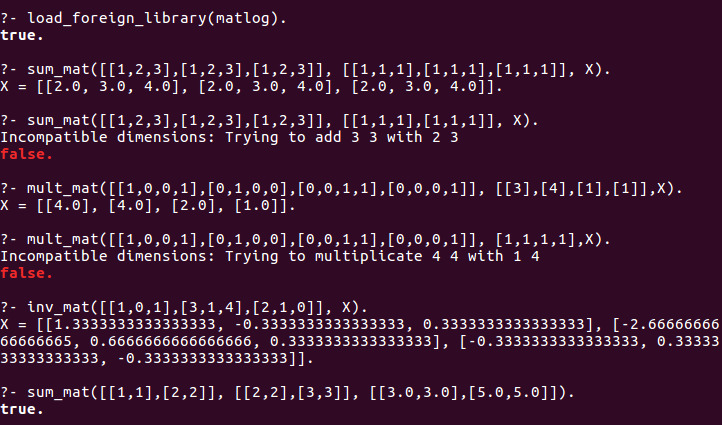
\includegraphics[scale=0.6]{Sesion.jpeg}

\section{Referencias}
\begin{flushleft}
[1] \href{http://www.swi-prolog.org/pldoc/man?section=foreign}{Foreign Language interface to C}.

[2] \href{http://www.swi-prolog.org/pldoc/doc_for?object=section('packages/pl2cpp.html')}{Foreign Language interface to C++}.\\
\end{flushleft}

\begin{lstlisting}[style=C++]
try {//In case the PlTail constructor fails
	PlTail list(term);	
   	PlTerm e1;

    while (list.next(e1)) { //Iterate over the list
       j = 0;
       PlTerm e2;
           PlTail list_row(e1);
           while (list_row.next(e2)) {
               content.push_back((double) e2);
               j++;
      		}   
    }
catch (...)
{
   std::cout << "Invalid matrix" << std::endl;
   return nullptr;
}
\end{lstlisting}

\end{document}

%%% Local Variables:
%%%   coding: utf-8
%%%   flyspell-mode: t
%%%   ispell-local-dictionary: "british"
%%% End:
